\documentclass[10pt]{article}
\usepackage[english]{babel}
\usepackage[utf8]{inputenc}
\usepackage[T1]{fontenc}
\usepackage{amsmath,amsfonts,amssymb,amsthm,cancel,siunitx,
calculator,calc,mathtools,empheq,latexsym}
\usepackage{subfig,epsfig,tikz,float}
\usepackage{booktabs,multicol,multirow,tabularx,array}
\usepackage{natbib}
\usepackage{graphicx}
\graphicspath{ {./images/} }
\setlength{\parindent}{0pt}
\setlength{\parskip}{5pt}
\textwidth 13.5cm
\textheight 19.5cm
\columnsep .5cm
\title{\renewcommand{\baselinestretch}{1.17}\normalsize\bf%
\uppercase{
	Studiul tehnicilor de recunoastere \\
	si clasificare a imaginilor 2D}
}
\author{
Barbu Vlad Alexandru$^{1}$, Stefanescu Gheorghe$^{2}$
}

\begin{document}

\date{}

\maketitle

\vspace{-0.5cm}

\begin{center}
{\footnotesize 
Facultatea de Matematica si Informatica, \\
Universitatea din Bucuresti, \\
Bucuresti, Romania \\
$^1$vlad.barbu@s.unibuc.ro \\
$^2$gheorghe.stefanescu@fmi.unibuc.ro \\
}
\end{center}

% -------------------------------------------------------------------
% Abstract
\bigskip
\noindent
{\small{\bf ABSTRACT.}
		Automatizarea clasificarii imaginilor si recunoasterea predictibila 
	a formelor de interes din contextul acestora reprezinta o problema complexa,
	avand implicatii majore in multe domenii stiintifice. Definirea unui
	proces sistematic de prelucrare, identificare si clasificare reprezinta
	un demers necesar abordarii acestei probleme. Acest raport incearca sa
	ofere o viziune de ansamblu asupra solutiilor existente, 
	avand drept obiect de studiu pentru analiza si implementarea acestora - recunoasterea 
	si extragerea informatiei din cadrul unui document scos la imprimanta (deseori pornind
	de la structura unui tipizat de baza, fiind completat ulterior in format digital
	sau cu scris de mana).
}

\medskip
\noindent
{\small{\bf Cuvinte cheie}{:} Recunoasterea formelor. Prelucrarea imaginilor. Clasificarea imaginilor 2D.
}

\baselineskip=\normalbaselineskip
% -------------------------------------------------------------------

\section{Introducere}\label{sec:1}

\> {\bf Procesul de recunoastere a formelor} poate fi vazut drept o inlantuire de proceduri cu ajutorul
carora se poate ajunge la un rezultat concludent de clasificare a unui obiect de
interes din cadrul unei multimi de entitati observabile. O astfel de metoda de recunoastere
devine utila mai ales atunci cand abordarea directa este imposibila - atunci cand o 
clasificare manuala nu este fezabila (in cazul in care nevoia de recunoastere este una recurenta).

\> {\bf Descrierea unui proces robust de clasificare automata a imaginilor} consta in
stabilirea unui set de reguli in baza caruia, datele de intrare pot fi grupate in clase
identificabile. O clasa identificabila este reprezentata de o multime finita de factori
cantitativi si calitativi cu ajutorul carora unui obiect observabil ii este asociat un numar de
atribute semnificative - contextul de identificare a unei astfel de clase este determinat de o colectie
predefinita de metadate. Metoda folosita pentru delimitarea claselor identificabile reprezinta un
caz particular specific domeniului de interes al aplicatiei concrete. 

\newpage

\section{Descrierea unui sistem de recunoastere}\label{sec:2}

\> Un sistem robust si eficient de recunoastere a formelor va oferi rezultate corecte, predictibile
urmand o inlantuire de proceduri de transformare, prelucrare, extractie si clasificare.
Componentele principale ale unui sistem de recunoastere si clasificare a formelor sunt urmatoarele:

\begin{itemize}
    \item {\bf Componenta de preprocesare} - cu ajutorul acestei componente se vor normaliza datele de intrare
	(mediul de provenienta al acestora fiind necunoscut, stabilirea unui standard este necesara)
	si se vor evidentia obiectele de interes prin eliminarea impuritatilor
	\item {\bf Selectorul de obiecte de interes} - in cadrul acestei etape, imaginea va fi parcursa
	si redusa la o multime de entitati de interes (structura observabilelor va fi definita
	prin intermediul acestei componente, urmand ca aceasta sa fie definitia standardului de metadate
	folosit de-a lungul procesului de recunoastere)
    \item {\bf Selectorul de atribute semnificative} - cu ajutorul acestuia, vom putea identifica
    factorii cantitativi si calitativi pe care un anumit observabil ii respecta (acesti factori trebuie sa fie predefiniti
	cu ajutorul unor descriptori relevanti domeniului de interes al aplicatiei)
    \item {\bf Componenta de masurare a atributelor} - responsabilitatea acestei componente este aceea de
    a calcula "importanta" atributelor asociate fiecarui observabil prin invocarea unui set
	predefinit de metrici si metode discriminative relevante pentru fiecare context de identificare, urmata
	de agregarea rezultatelor obtinute
    \item {\bf Clasificatorul} - etapa finala a procesului de recunoastere este reprezentata de
    efectuarea unei alegeri prin compararea masuratorilor efectuate in pasii anteriori pentru fiecare clasa
	identificabila predefinita
\end{itemize}

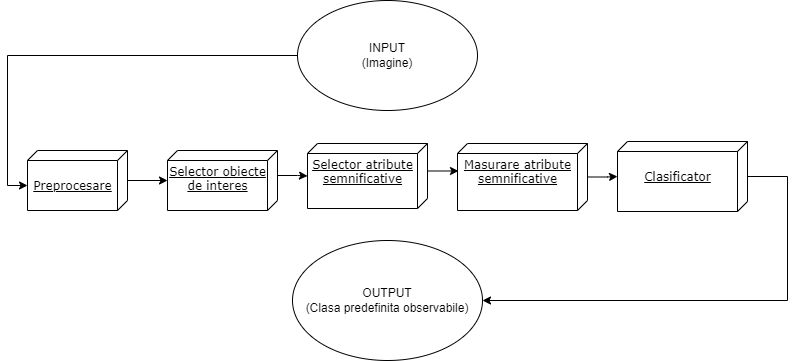
\includegraphics[scale=0.5]{componente}


\newpage

\section{Componenta de preprocesare}\label{sec:3}



\end{document}
